\documentclass{beamer}
%\usepackage{amsfonts,amsmath,oldgerm}
\usepackage{listings}
\usepackage{tcolorbox}
\usepackage{ulem}
\usepackage{algpseudocode}
\usepackage[T1]{fontenc}
\usepackage[utf8]{inputenc}
\usepackage{amsmath}

\usepackage[vlined, linesnumbered]{algorithm2e}

\usepackage{booktabs} 
\usepackage{caption}

\usepackage{tikz}
\usetikzlibrary{shapes.geometric, arrows, positioning}

\tikzstyle{box} = [
    rectangle, 
    minimum width=2.5cm, 
    minimum height=1.2cm, 
    text centered, 
    text width=2.5cm, 
    draw=black, 
    top color=white, 
    thick
]

\tikzstyle{arrow} = [
    ultra thick, 
    ->, 
    >=stealth, 
    gray!80
    %-triangle 60
]

\usetheme{ufrgs}
% \usepackage[sfdefault]{atkinson}

\newcommand{\testcolor}[1]{\colorbox{#1}{\textcolor{#1}{test}}~\texttt{#1}}
\newcommand{\starflet}{\textbf{Star-Fletcher}}
\newcommand{\waveprop}{\texttt{wave\_propagation}}
\newcommand{\waveinsert}{\texttt{wave\_insertion}}
\newcommand{\blockwrite}{\texttt{write\_block}}

% \usefonttheme[onlymath]{serif}

% \useoutertheme{miniframes}
\graphicspath{ {./images/} }
\titlebackground*{rtm}


\newcommand{\hrefcol}[2]{\textcolor{cyan}{\href{#1}{#2}}}

\title{Tarefas e Fletcher}
\subtitle{Implementação das equações de Fletcher usando um modelo de tarefas.}
\author{\href{mailto:phbcolle@inf.ufrgs.br}{Pedro Henrique Boniatti Colle}}
\date{Apresentação do Seminário de Andamento -- 23/11/26}

\begin{document}
\maketitle


% Objetivos
% - Introduzir bem os elementos de pesquisa
%   - O que é RTM
%   - O que é STF
% - Como foi a implementação do algoritmo
%   - Segmentação do espaço
%   - Rediscretização do tempo
%   - 1 slide para cada task
% - Resultados Preliminares
% - Conclusão

\section{Introdução}

\begin{frame}{Contexto}
  \begin{itemize}
  \item<+-> \textit{High performance Computing} já é um campo complexo.
  \item<+-> Com o crescimento de IA, há o surgimento de novos aceleradores.
    \begin{itemize}
    \item CPU
    \item GPU
    \item FPGAs
    \item TPUs
    \item Hardware Especializado
    \end{itemize}
  \item<+-> Como usar todo o poder de processamento de um parque de alta performance?
  \item<.-> Faz sentido usarmos apenas a GPU nos nodos do parque?
  \item<.-> Porque não todos os recursos?
  \end{itemize}
\end{frame}

\begin{frame}{Sequential Task Flow}
  \begin{itemize}
  \item<+-> \textit{Sequential Task Flow} (STF) é uma técnica de divisão de trabalho em \textbf{tarefas}.
  \item<+-> Essas \textbf{tarefas} podem depender da conclusão de outras tarefas para executar, formando um DAG.
  \item<+-> Elas são submetidas sequencialmente e a relação entre as dependências é determinada pelo \textit{runtime}. 
  \end{itemize}
  \uncover<4>{
    \centering
    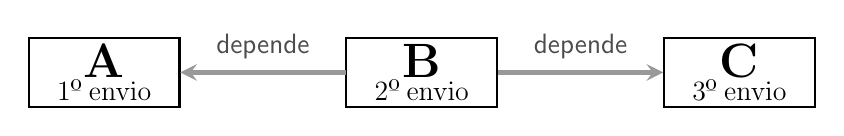
\begin{tikzpicture}[scale=0.7, transform shape]
    
    % Nodes
    \node (B) [box] {\Huge\textbf{B} \\ \Large 2º envio};
    \node (A) [box, left=3cm of B] {\Huge\textbf{A} \\ \Large 1º envio};
    \node (C) [box, right=3cm of B] {\Huge\textbf{C} \\ \Large 3º envio};
    
    % Edges with text
    \draw [arrow] (B.west) -- (A.east) node[midway, sloped, above=0.1cm, font=\Large\sffamily, color=black!70] {depende};
    \draw [arrow] (B.east) -- (C.west) node[midway, sloped, above=0.1cm, font=\Large\sffamily, color=black!70] {depende};
    
    \end{tikzpicture}
  }
\end{frame}

\begin{frame}{StarPU}
  \begin{itemize}
  \item StarPU é um desses runtimes de STF.
  \item Gerência dependências de dado e memória automaticamente.
  \item Permite vários escalonadores diferentes.
  \item Fácil adição de diferentes fontes de execução de código.
  \end{itemize}
\end{frame}


\begin{frame}{Multiplos Executores}
  \begin{figure}[ht]
    \centering
    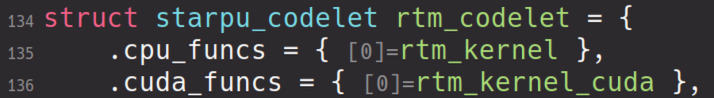
\includegraphics[width=0.8\textwidth]{codelet.png}
  \end{figure}
  \begin{itemize}
  \item Implementação de um \textit{codelet} com dois executores: em CPU e em GPU.
  \item Os diferentes escalonadores são capazes de distribuir a carga entre os possíveis locais de execução.
  \end{itemize}
\end{frame}

\begin{frame}{Fletcher}
  \begin{itemize}
  \item<+-> As \textit{Equações do Fletcher} são equações que modelam o meio TTI (Tilted Transversely Isotropic) usadas na analise de depósitos de óleo e gás no pré-sál.
  \item<.-> Há uma versão implementada pelo Gabriel Freytag. Inicialmente desenvolvido pelo Nesi.
  \end{itemize}

  \begin{figure}[ht]
    \centering
    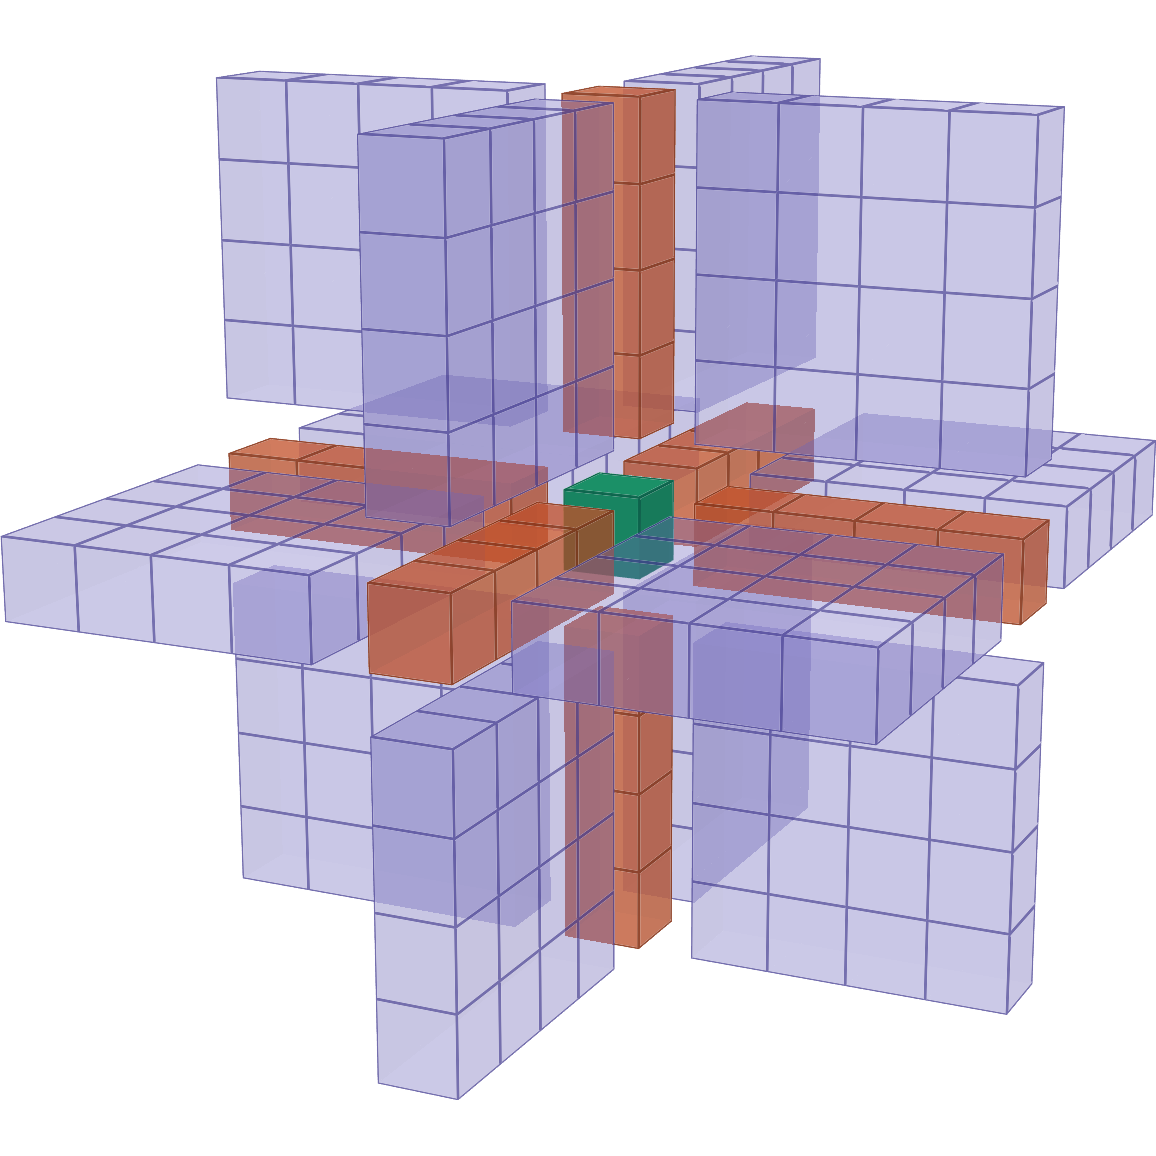
\includegraphics[width=0.3\textwidth]{stencil.png}
  \end{figure}

\end{frame}

\begin{frame}{Funcionamento}
  \begin{itemize}
  \item<+-> É a discretização de equações diferenciais de onda.
  \item<.-> Trabalha-se com a onda primária e secundária.
  \item<.-> Realiza-se duas etapas:
    \begin{itemize}
    \item<+-> Propaga-se a onda gravada, salvando a cada $k$ passos.
    \item<+-> Lê-se a onda gravada a cada $k$ passos, propagando a onda no sentido contrário ao tempo.
    \end{itemize}
  \item<+-> Esse processo é chamado de \emph{shot} e gera uma imagem subsuperficial parcial.
  \end{itemize}
\end{frame}

\begin{frame}{Funcionamento}
  \begin{itemize}
  \item<+-> A versão base, do Nesi, foca-se apenas na etapa na \textit{forward}, salvando o meio a cada $k$ passos em disco.
  \item<.-> Focando apenas nas computações dentro de um \textit{shot}
  \item<+-> Nos baseamos nele para construir a nossa versão..
  \end{itemize}
\end{frame}

\begin{frame}{Limitações}
  \begin{itemize}
  \item<+-> Os volumes de dados podem ser enormes.
  \item<.-> Um volume de $1024 \times 1024 \times 512$ salvo em ponto fluante de dupla precisão consite em $4Gb$.
  \item<.-> Logo, o processo de salvar a cada $k$ passos e depois ler nessa mesma taxa é muito custoso.
  \item<+-> O algoritmo é \textbf{I/O bound}.
  \item<+-> Muito esforço tem que vir do programador para gerir essas transfências de dados e maximizar o processamento das máquinas.
  \item<.-> Há pesquisas dos outros labs sobre isso.
  \item<.-> Além disso, com um volume grande o suficiente, computação em um único nodo não é viável.
  \end{itemize}
\end{frame}


\begin{frame}{\starflet}
  \begin{itemize}
  \item<+-> O meu trabalho apresenta \starflet.
  \item<.-> Uma implementação do Fletcher usando STF em primeira ordem. 
  \item<.-> Baseado na implementação do Nesi.
    \begin{itemize}
    \item<+-> O espaço é segmentado em blocos.
    \item<+-> Cada tarefa, distribuida aos trabalhadores, é de computar um dos blocos.
    \item<+-> Cada iteração depende das anteriores.
    \item<+-> É possível submeter todas as tarefas enquanto o código executa, sem problemas de sincronização.
    \end{itemize}
  \item<+-> Modelar com o StarPU permitiu \textbf{naturalmente} gerar a quebra das iterações e do \textit{weaving} do I/O.
  \end{itemize}
\end{frame}


\section{Implementação}

\begin{frame}[fragile]{Implementação do Baseline}
  \begin{itemize}
    \item Começou-se da implementação do Nesi.
    \item Modelo Fork-Join para OpenMP.
    \item Implementação em CUDA também.
  \end{itemize}

\scriptsize
  \begin{algorithm}[H]
    \SetAlgoLined
\DontPrintSemicolon
\SetKwFunction{FSource}{Source}
\SetKwFunction{FInsert}{InsertSource}
\SetKwFunction{FPropagate}{Propagate}
\SetKwFunction{FSwap}{SwapArrays}
\SetKwFunction{FDump}{WriteVolume}

\SetKwInOut{Input}{Input}
\Input{Ondas $pc, qc, pp, qp$, Iterações totais $st$, Escrita a cada $k$}

\BlankLine
\For{$t \longleftarrow 1$ \KwTo $st$}{
  \FInsert{$pc, qc$}\;
  \tcp{Função Paralela}
    \FPropagate{$pp, pc, qp, qc$}\;
    \FSwap{$pp, pc, qp, qc$}\;
    \If{$t \bmod k = 0$}{
      \FDump{$pc$}\;
    }
}
  \end{algorithm}


\end{frame}

\begin{frame}{Desafios}
  \begin{itemize}
  \item<+-> Desafios de implementação:
    \begin{enumerate}
    \item<+-> Segmentar em blocos.
    \item<.-> Realizar a comunicação inter-bloco.
    \item<.-> Quebrar a dependência de dados de iterações.
    \item<.-> Rediscretização do espaço das iterações.
    \end{enumerate}
  \end{itemize}
\end{frame}

\begin{frame}[fragile]{Segmentação Espacial}
  \begin{itemize}
    \item Comunicação inter-bloco adiciona \textit{checks}.
    \item Aumenta o volume de dados por segmento.
  \end{itemize}
  \begin{figure}[ht]
      \centering
      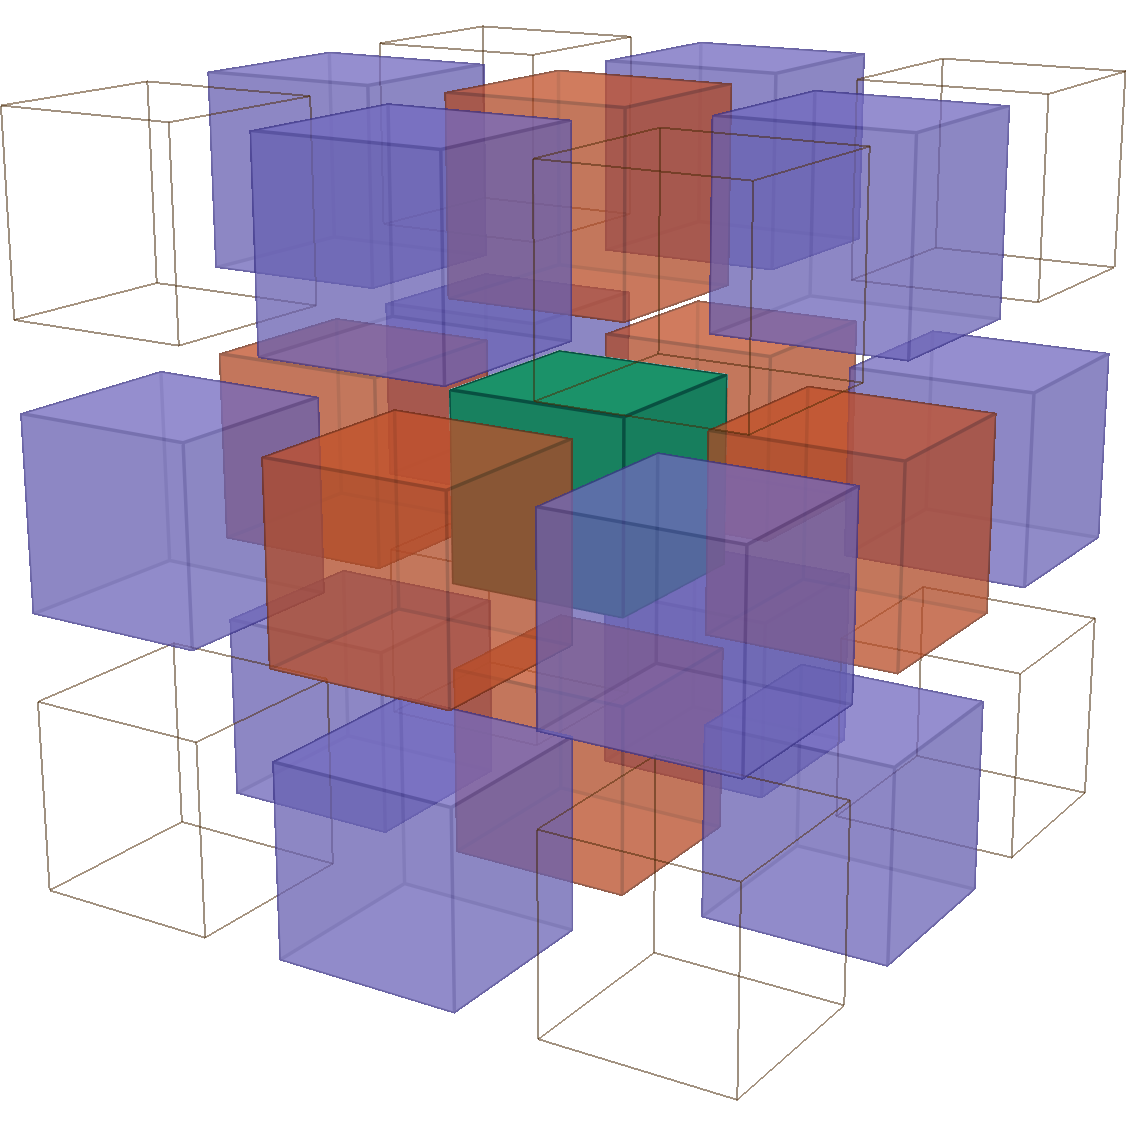
\includegraphics[width=0.35\textwidth]{neighbors.png}
  \end{figure}

\end{frame}

\begin{frame}{Segmentação Espacial}
  \begin{itemize}
    \item<+-> Implementação atual se demonstrou muito boa para a computação em CPU.
    \item<+-> Porém não escalou bem para GPU.
    \item<.-> Cada bloco precisa dos seus 18 vizinhos.
    \item<.-> Usando o \texttt{nvidia-smi} observou-se que a GPU ficava em 50\% enquanto o throughput de dados estava em 100\%.
    \item<+-> Trabalha-se atualmente em um redisign para melhor aproveitar a GPU.
  \end{itemize}
\end{frame}

\begin{frame}{Rediscretização Espacial}
  \begin{itemize}
  \item<+-> Como visto no pseudocódigo, a verão base alterna entre dois buffers.
  \item<.-> Isso segura as execuções e limita quantas tarefas podem ser executadas, criando um ponto de sincronização desnecessário no contexto de tarefas.
  \item<+-> Nisso transformou-se o antigo processo de swap.
    \begin{align*}
       P_c &\leftarrow F(P_p) - P_c \\
       P_c &\;swap\; P_p
    \end{align*}
  \item<.-> Para:
    \begin{align*}
      P_t  &\leftarrow F(P_{t-1}) - P_{t-2} 
    \end{align*}
    
  \end{itemize}
\end{frame}

\section{Resultados Parciais}

% TODO: resultados parciais tem que ser extraído de tudo que foi obtido.


\begin{frame}{Resultados: Desempenho em CPU}
  \begin{itemize}
  \item Comparação com o \textit{fletcher-base} (OpenMP) em 6 máquinas CPU, métrica MSamples/s.
  \item \starflet{} supera a melhor configuração do baseline em 3 máquinas
  \item Contra o \textit{schedule} estático padrão, ganho de 63\% nas máquinas híbridas (P/E-cores).
  \end{itemize}
\end{frame}

\begin{frame}{Desempenho em CPU}
    \begin{figure}[ht]
        \centering
        % trim order: Left, Bottom, Right, Top
        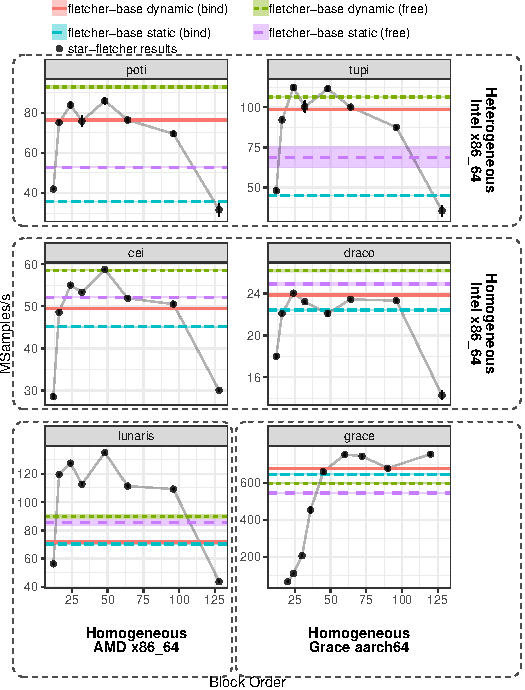
\includegraphics[page=1, trim=0pt 305pt 0pt 0pt, clip, width=0.6\textwidth]{msamples.pdf}

        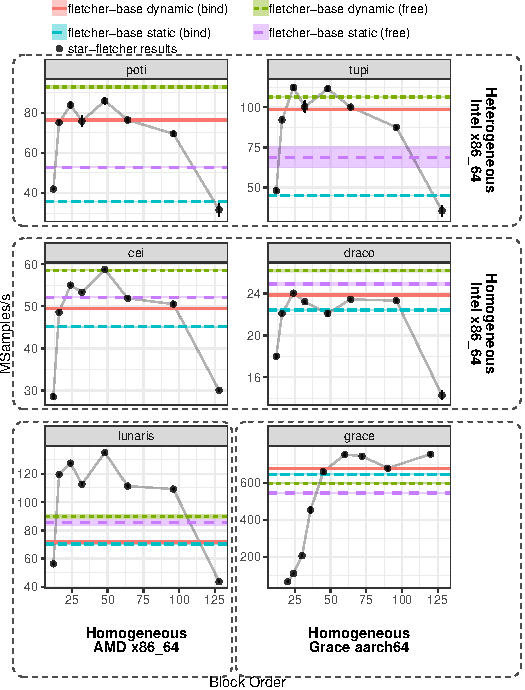
\includegraphics[page=1, trim=0pt 221pt 0pt 26pt, clip, width=0.49\textwidth]{msamples.pdf}
        \hfill
        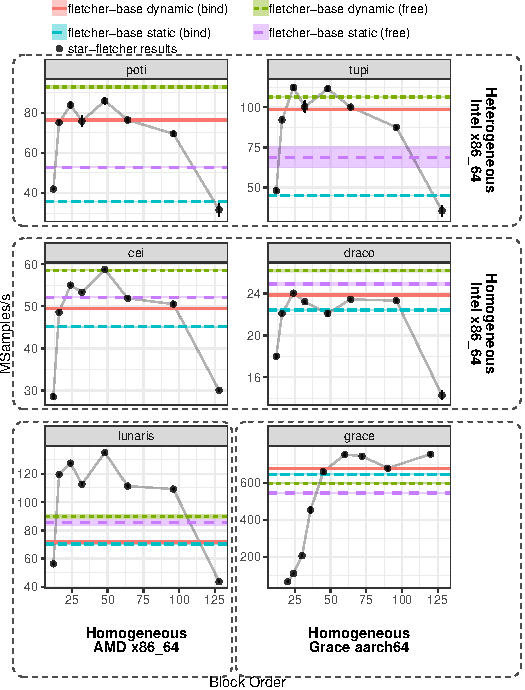
\includegraphics[page=1, trim=0pt 134pt 0pt 112pt, clip, width=0.49\textwidth]{msamples.pdf}
    \end{figure}
\end{frame}

\begin{frame}{Desempenho em CPU}
    \begin{figure}[ht]
        \centering
        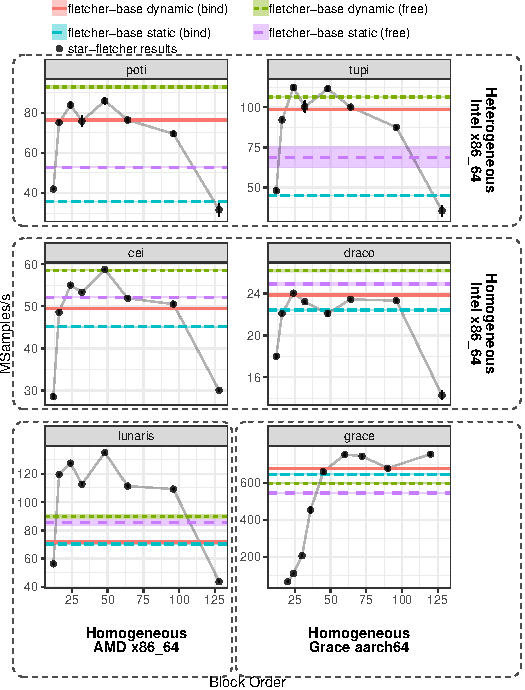
\includegraphics[page=1, trim=0pt 305pt 0pt 0pt, clip, width=0.6\textwidth]{msamples.pdf}

        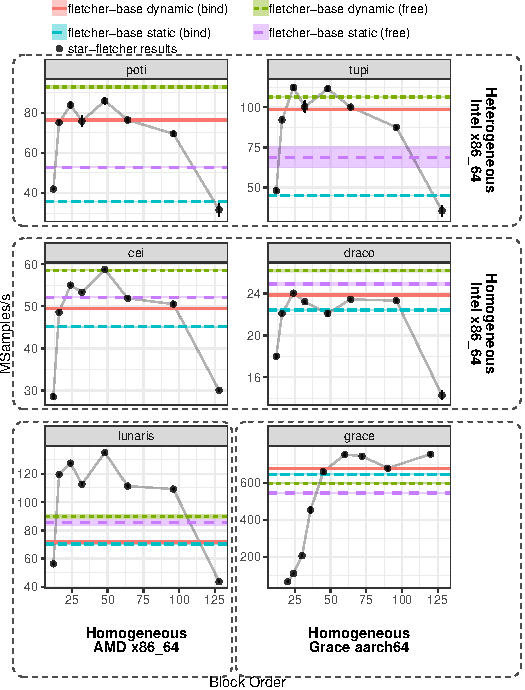
\includegraphics[page=1, trim=0pt 0pt 0pt 199pt, clip, height=0.65\textheight]{msamples.pdf}
    \end{figure}
\end{frame}

\begin{frame}{Sobreposição de Iterações}
  \begin{itemize}
  \item Sem a barreira global, até 7 iterações executam ao mesmo tempo.
  \item O I/O é intercalado com a computação, em vez de bloquear a iteração seguinte.
  \item Usamos \texttt{mmap} para fazer um volume final igual e isso fica lento em volumes maiores.
  \end{itemize}
\end{frame}

\begin{frame}{Sobreposição de Iterações}
    \begin{figure}[ht]
        \centering
        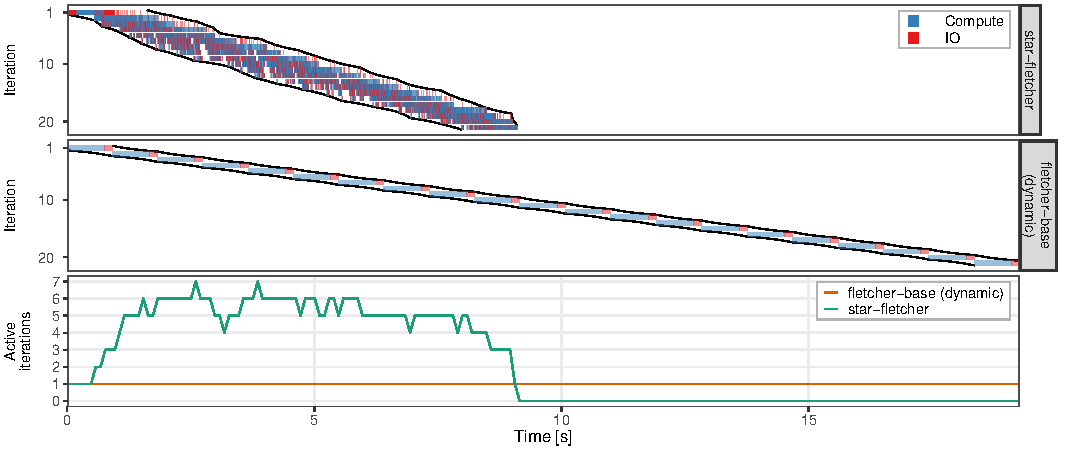
\includegraphics[width=\textwidth, height=0.85\textheight, keepaspectratio]{overlap.pdf}
    \end{figure}
\end{frame}

\begin{frame}{Desempenho em GPU}
  \begin{itemize}
  \item<+-> Em GPU, os resultados ainda não são satisfatórios.
  \item Para todas as máquinas e escalonadores, \starflet{} fica muito abaixo do \textit{fletcher-base}.
  \item Na \texttt{tupi}, o melhor caso chega a $\sim$1000 MSamples/s, contra $\sim$8000 do baseline.
  \item<+-> Consistente com o gargalo de transferência dos 18 vizinhos de cada bloco.
  \end{itemize}
\end{frame}

\begin{frame}{Desempenho em GPU}
    \begin{figure}[ht]
        \centering
        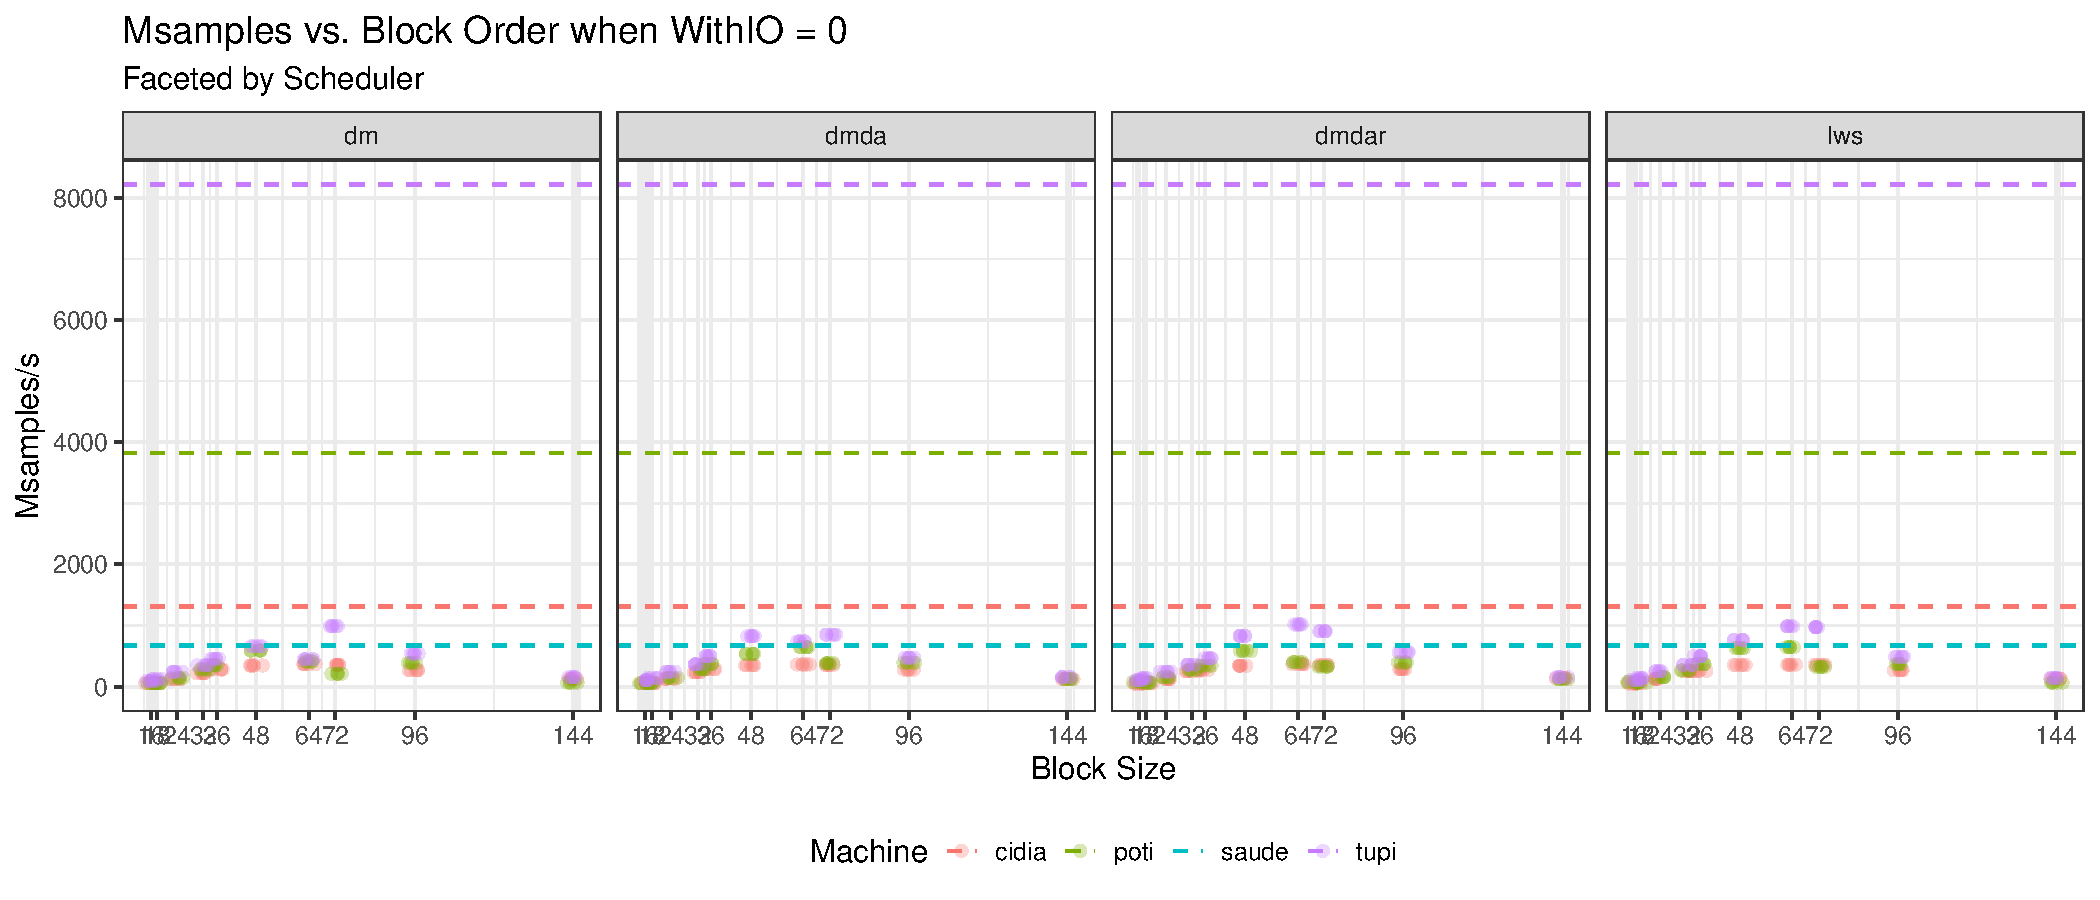
\includegraphics[width=\textwidth, height=0.85\textheight, keepaspectratio]{ideal-seg-msamples.pdf}
    \end{figure}
\end{frame}

\section{Conclusão}

\begin{frame}{Conclusão}
  \begin{itemize}

  \item<+-> O modelo STF com StarPU se mostrou vantajoso em CPU.
    \begin{itemize}
    \item<.-> \starflet{} é competitivo com o \textit{fletcher-base}, pricipalmente nas máquinas de HPC mais modernas.
    \item<.-> Sem a barreira global, iterações se sobrepõem e o I/O é intercalado com a computação.
    \end{itemize}
  \item<+-> Ainda há limitações:
    \begin{itemize}
    \item<.-> A escrita via \texttt{mmap} fica lenta em volumes maiores.
    \item<.-> Em GPU, o desempenho ainda está muito abaixo do baseline, limitado pela transferência dos vizinhos de cada bloco.
    \end{itemize}
  \end{itemize}
\end{frame}

\begin{frame}{Publicações}

  \begin{itemize}
    \item<+-> Publicações solo.
    \begin{itemize}
      \item<.-> Pequena publicação no ERAD-RS.
      \item<.-> REJECT no SSCAD.
      \item<.-> Submission no PDP.
    \end{itemize}
    \item<+-> Publicações do Lab.
    \begin{itemize}
      \item<.-> Publicação no CARLA sobre ferramentas de ensino de Programação Distribuida e Paralela.
      \item<.-> Publicação no UCC sobre o uso de simulações para model Cloud Offloading.
      \item<.-> Trabalhando em um artigo para o CCGRID sobre o mesmo assunto.
    \end{itemize}
  \end{itemize}
\end{frame}

\begin{frame}{Metas Atuais}
  \begin{itemize}
    \item<+-> Refazer uma partição de blocos mais favorável a GPU
    \begin{itemize}
      \item<.-> Implementação de Halo
      \item<.-> Implementação de \textit{parallel workers} para a CPU
    \end{itemize}
    \item<+-> Com resultados satisfatórios, mover para MPI
    \item<.-> Avaliar comparativamente com o trabalho do Spadotto.
  \end{itemize}
\end{frame}


\backmatter
\end{document}
